\section{Discovery: an architectural proposal}
\label{sec:architecture}

\subsection{Related work}

\begin{itemize}

	\item Moreno made a proposition of IaaS architecture \cite{moreno2012iaas}.	
	
	\item He identified a list of services that are vital for building IaaS that will be usable in production condition for commercial company.

	\item We aim at making a research prototype: we want to keep concepts that are vital for a first prototype:

		\begin{description}

			\item [Virtual Machine] : Prototype will enable reasearchers to access a big compute power.

			\item [Virtual Network] : In addition to infrastructure network, we want to connect virtual machines on an isolated network.

			\item [Image disk and persistent storage] : 
				\begin{itemize}

					\item Virtual machines will be based on images

					\item Virtual machines' states are savable.
				
				\end{itemize}

			\item [Simple authentication] : User will have to authenticate to access prototype. Once they are authenticated they will be able to create virtual machines.

		\end{description}

\end{itemize}

\subsection{First iteration on the LUC-OS architecture}

\begin{itemize}

	\item For our first iteration, we keep 4 main services:
		\begin{description}

			\item [Compute manager] : responsible for virtual machines lifecycle.

			\item [Network manager] : responsible for virtual networks.

			\item [Storage manager] : responsible for images and persistent block storage.

			\item [Administrative manager] : responsible for infrastructure management and user permissions.  

		\end{description}


	\item In figure \ref{fig:mcd} we propose a conceptual data model to explain our proposal.


	\begin{figure*}
		\centering
		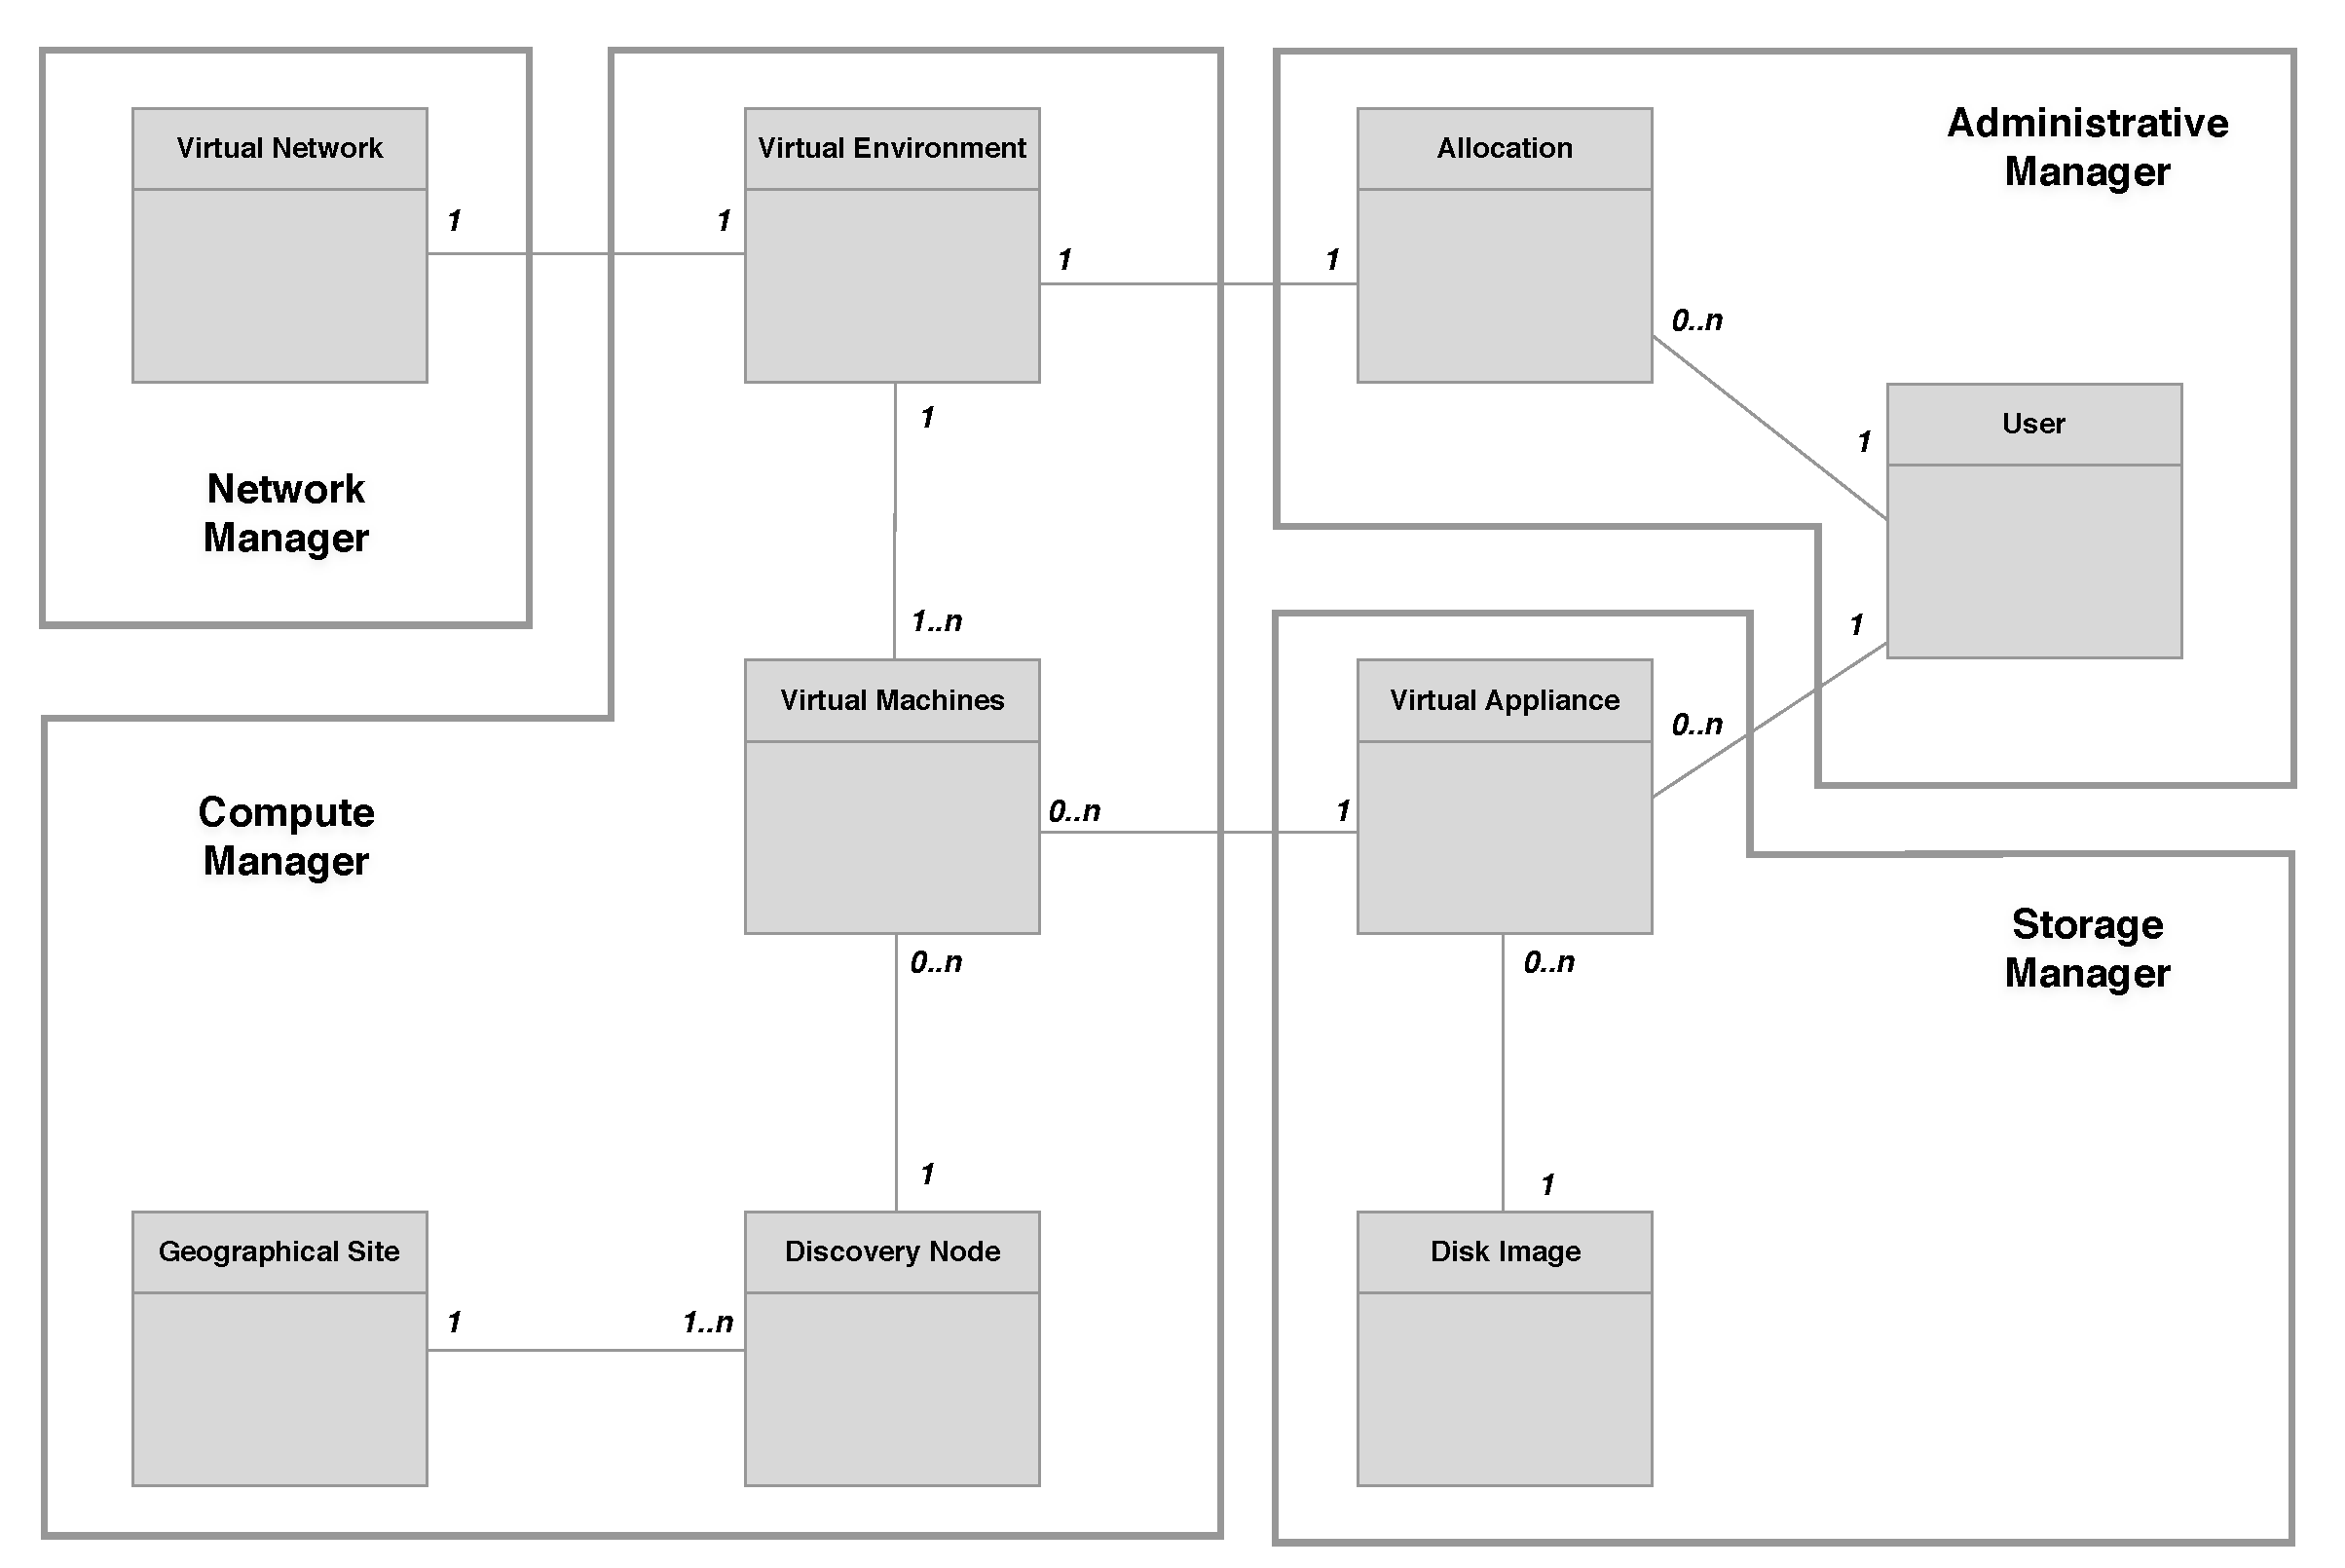
\includegraphics[width=0.91\linewidth]{Figures/mcd_3.pdf}
		\caption{Conceptual Data Model for Discovery proposal.}%
		\label{fig:mcd}%
		%\vspace*{-.8cm}
	\end{figure*}

	\item Virtual environment concept is the keystone of the Discovery proposal:
		
		\begin{itemize}

			\item When a user request the creation of virtual machines for a specified date, an allocation is registered.

			\item When the start date is reached, a virtual environment (isolated container for a VLAN and VMs) is created.

			\item a virtual environment can be run on several hosts, possibly spread over several geographical sites.

		\end{itemize}

	\item + description of other entities.

\end{itemize}